\chapter{Analyse des opportunités des technologies libres dans
le domaine de l'édition vidéo et prévisions}
\minitoc \mtcskip \newpage

\paragraph{}
Maintenant que les besoins et que les solutions existantes
ont été analysées on rendra compte de la
situation actuelle des technologies libres, de leurs communautés. Il est
aussi important de chercher les raisons qui expliquent que ces
logiciels ne sont pas utilisés par les professionnels. Puis, nous essayerons
d'envisager les solutions possibles qui permettraient de remédier à ce
situation.

\paragraph{}
Dans cette partie, nous analyserons la différence entre les
manières d'envisager la création de logiciel et nous verrons quels sont les
avantages et inconvénients de ces fonctionnements. Par la, suite nous
nous concentrerons sur les frameworks existants pour faire une analyse
technique des ces technologies. Par la suite, nous analyserons
les communautés qui portent ces différents projets afin d'arriver à
voir les lacunes et les avantages de chacun des projets.  Pour finir,
nous tirerons les conclusions de cette analyse afin de trouver des
solutions aux défis qu'est la création d'un logiciel libre de montage
vidéo.

\newpage
\begin{figure}
  \begin{center}
    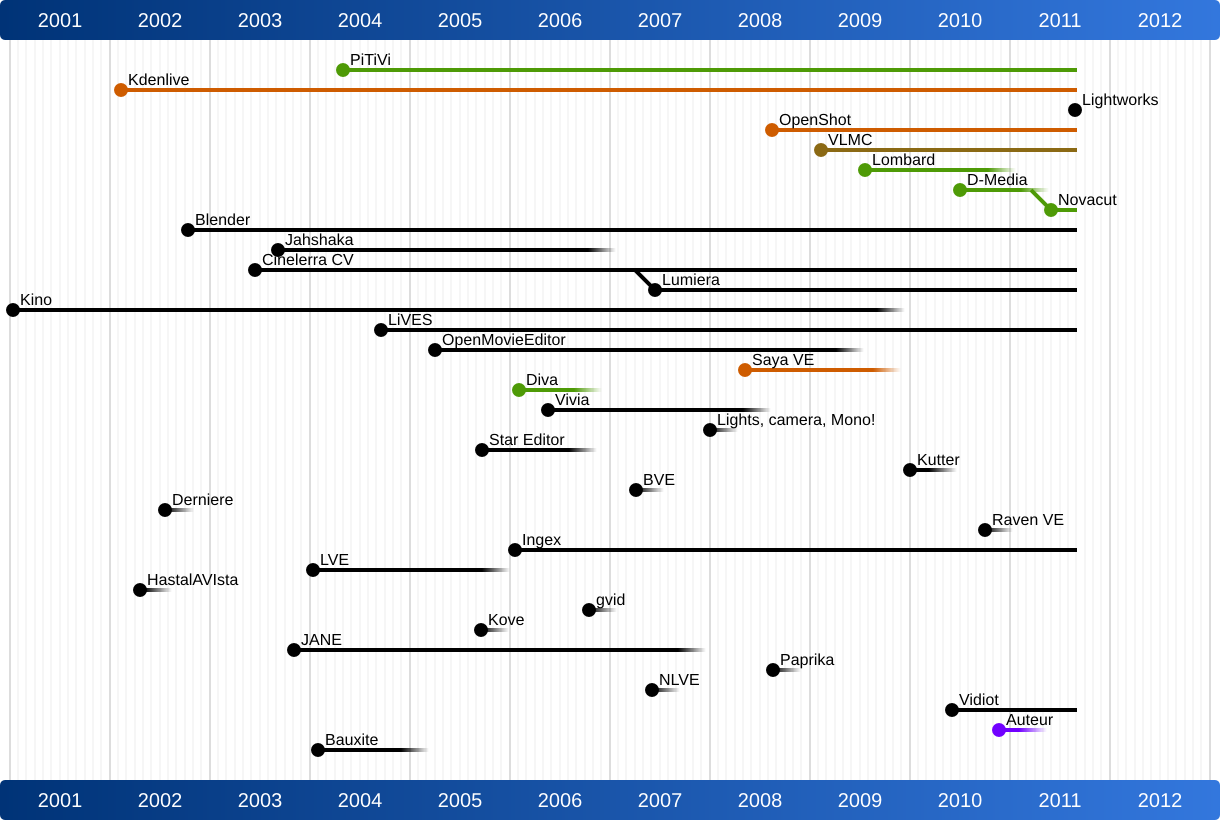
\includegraphics[width=0.9\textwidth]{images/open-source-video-editor-timeline}
  \end{center} \caption{Open source video editors timeline} \label{Yes}
\end{figure}

\paragraph{}
A l'heure actuelle, il existe un nombre réduit de projets qui
sont plus ou moins matures, mais des projet issus du monde propriétaire
sont en train de faire la transition vers la libération de leur code
\cite{TheLightworksOpenSourceProjectStartHere}. Cela fait plus d'un an que
le projet de libération de lightworks a été lancé mais la libération
du code n'a toujours pas eu lieu. Il ne sera donc pas possible d'analyser
le produit de manière technique, et il conviendra de le faire au moment
où le code sera effectivement publiquement visible.

\section{Technologies} \paragraph{} Pour faire une analyse technique
des produits permettant de faire de l'édition vidéo, il est nécessaire
d'analyser le ``core'' des logiciels, c'est à dire la partie du
logiciel où les opérations d'édition sont effectivement réalisées. Dans
ce domaines, il existe deux façon de procéder dans le monde de l'édition
vidéo open source.

\begin{itemize}
  \item{La première est de réaliser à la fois la partie graphique et
    les calculs permettant la gestion de l'édition non linéaire au
    sein d'une même entité de code. Le résultat de cela est un logiciel
    monolithique. Le logiciel Cinelerra est un %FIXME
    exemple dans lequel les développeurs ont décidé d'utiliser ce
    mode de fonctionnement.}
  \item{La deuxième est d'utiliser/créer un framework\footnote{Un
    framework est un ensemble d'outils et de composants logiciels
    organisés conformément à un plan d'architecture et des design
    patterns. L'ensemble forme un squelette de programme.}, et d'ensuite
    créer une interface graphique utilisant ce cadre logiciel. La
    plupart des logiciels libres ont suivi ce plan de conception. Le
    logiciel PiTiVi utilise le Framework multimedia GStreamer alors que
    KDEnlive utilise le framework orienté édition et broadcasting
    MLT. Dans le cadre des Frameworks, nous nous intéresserons en
    particulier à l'analyse de ceux-ci puisque les notions relatives à
    l'édition vidéo, et la gestion de toute la partie multimédia est
    réalisée par ceux-ci. Les logiciels d'édition ne sont à priori
    que de simples interfaces graphiques basées sur ces frameworks,
    et par conséquent leur analyse ne présente qu'un faible intérêt.}
\end{itemize}

\section{Logiciel monolithique} %FIXME Look for a def

\paragraph{} Par le terme logiciel monolithique, il convient de
comprendre que le logiciel peut utiliser des librairies externes, mais
le core de ce même logiciel, et la logique d'édition linéaire à
proprement parler est directement faite à l'intérieur du logiciel et
non par une librairie où framework externe. Cela a pour principal avantage
que la conception est simplifiée pour plusieurs raisons à savoir:

\begin{itemize}
  \item {Les développeurs n'ont pas la nécessité de penser
    en terme d'interface publique de programmation (API),
    et n'ont pas à garantir la stabilité de celle-ci. Cela
    a pour effet que la qualité de l'architecture
    risque de ne pas être optimale puisque la création d'API oblige
    les développeurs/architectes à réellement analyser les besoins
    de manière plus large dès le début de la conception. Dans le cas
    où l'on ne crée pas d'interface publique de programmation voué à
    être réutilisée, le risque est que le travail de design et
    d'architecture ne soit pas réalisé.}
  \item {Les développeurs n'ont besoin de penser l'architecture que pour
    les seuls cas d'utilisation qui sont liés à ce même logiciel, %FIXME citations 
    ils n'ont pas à voir au delà de ces use cases.}
  \item {Les erreurs en terme de design n'ont pas d'incidences aussi graves
    que dans le cas d'un framework.}
\end {itemize}

\paragraph{} On se rend compte que cette manière de faire a pour
principal avantage le fait que le logiciel peut être développé plus
rapidement puisque le core du logiciel, et donc le code qui implémente
la logique de l'édition non linéaire est conçue avec pour seul cas
d'utilisation, celui du logiciel. Cependant, de
nombreux inconvénients existent de par la nature monolithique du design:

\begin{itemize}
  \item{TODO}
\end{itemize}

\paragraph{} De plus, afin d'implémenter un logiciel de montage vidéo
dans son ensemble, le code à produire est considérable, comme
le montre les statistiques (Annexes 2). Le logiciel Cinelerra à lui
seul fait plus d'un million de lignes. Une telle quantité de code est
difficile à maintenir et requiert des ressources importantes en terme
de main d'oeuvre.

\paragraph{} L'un des inconvénients de cette manière de faire est que
le code que l'on a à l'intérieur du logiciel n'est pas réutilisable
directement par d'autres projets, et par conséquent, on peut considérer
que cela est ``individualiste``, chose qu'il convient d'éviter dans le
cadre du développement de logiciel libre afin de ne pas multiplier les
efforts, et dupliquer le code.

\paragraph{} Cette façon de faire a été utilisée par le projet
Cinelerra. Ce logiciel est le plus avancé en terme de fonctionnalités
que le marché des logiciels libres de montage offre. On peut
penser que son architecture monolithique expliquer ce développement
plus abouti. Bien qu'il y ait évidemment de nombreux autre facteurs. TODO


\section{Analyse technique}

\section{Analyse des communauté}

\section{Lacunes}

\section{Solutions possibles}
